\documentclass[11pt]{article}

\usepackage[margin=1in]{geometry}
\usepackage{setspace}
\onehalfspacing
\usepackage{graphicx}
\graphicspath{report_images/}
\usepackage{appendix}
\usepackage{listings}

% DOCUMENT INFORMATION =================================================
\title {ECEN 429: Introduction to Digital Systems Design Laboratory \\ North Carolina Agricultural and Technical State University \\ Department of Electrical and Computer Engineering} % Declare Title
\author{Reporter: Chris Cannon \\ \and Partner: Nikiyah Beaulah} % Declare authors
\date{February 1, 2018}
% ======================================================================

\begin{document}

\maketitle % Render Title, Author, and Date

\begin{center}
Lab	1
\end{center}

\pagebreak

\section{Introduction}
For this first lab our task was to familiarize ourselves with Xilinx Vivado Design Suite and the Digilent Basys3 FPGA Development Board that is used in this lab. During these tasks we learned how to configure the settings on Vivado for our board and how to load a program to the board. We also have three programming assignments for this lab. The first assignment was to write a simple VHDL program using an AND gate with two inputs and one output. The second assignment was to write a VHDL program using the car alarm example which that we derived in class. Our car alarm consists of 3 inputs using switches and 2 outputs using LED lights.  The third assignment was to create our own design implementation and write a VHDL program using only 4 inputs and 3 outputs. For our third assignment, we elected to build an adder for two 2-bit numbers. Upon successfully completing this lab, we will be able to work comfortable translating our circuit designs and VHDL code to a Vivado project and implement it on the Basys3 board.

\section{Background, Design Solution, and Results}
\subsection{Problem 1: 2-bit AND Gate}
The objective of this problem is to implement a single 2-bit AND gate and a single 2-bit OR gate in VHDL using the Basys3. The circuit diagram for this problem is in Figure 1.

\subsubsection{Background and Design Solution}

\begin{figure}[h]
	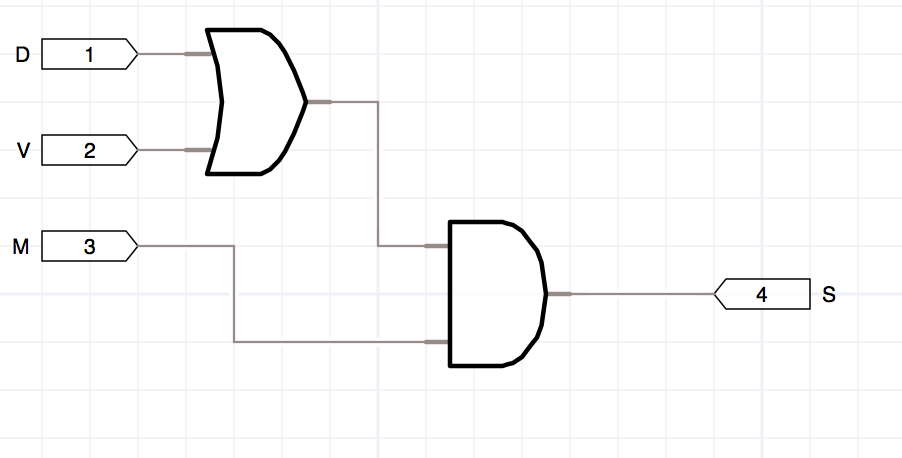
\includegraphics[width=\textwidth]{report_images/img2}
	\caption{\label{fig:figure-name}Circuit diagram for AND gate.}
\end{figure}

The inputs for this problem are labeled as 'A', 'B', and 'C'. The outputs are labeled 'D' and 'E'. The outputs are the product of an AND gate and an OR gate, respectively. This is demonstrated by the truth table shown in Table 1. The assignments for these pins were given by the instructions, and are shown in Table 2.

\begin{table}[h]
\begin{center}
	\begin{tabular}{| l | l | l | l | l |}
		\hline
		A & B & C & D & E \\ \hline
		0 & 0 & 0 & 0 & 0 \\ \hline
		0 & 0 & 1 & 0 & 1 \\ \hline
		0 & 1 & 0 & 0 & 1 \\ \hline
		0 & 1 & 1 & 0 & 1 \\ \hline
		1 & 0 & 0 & 0 & 0 \\ \hline
		1 & 0 & 1 & 0 & 1 \\ \hline
		1 & 1 & 0 & 1 & 1 \\ \hline
		1 & 1 & 1 & 1 & 1 \\ \hline
	\end{tabular}
	\caption{\label{tab:table-name}Truth Table for Problem 1.}
\end{center}	
\end{table}

\begin{table}[h]
\begin{center}
	\begin{tabular}{| l | l | l |}
		\hline
		Bit & Label & Address\\ \hline
		A & Switch 0 & V17 \\ \hline
		B & Switch 1 & V16 \\ \hline
		C & Switch 2 & W16 \\ \hline
		D & LED 7 & V14 \\ \hline
		E & LED 6 & U14 \\ \hline
	\end{tabular}
	\caption{\label{tab:table-name}Input and output bit specifications for problem 1.}
\end{center}
\end{table}

\subsubsection{Results}

This design functioned very easily, and we were able to observe each output 'C' for every combination of 'A' and 'B'. They are shown in Figure PICS. 

\subsection{Problem 2: Car Alarm}

Problem 2 referenced a car alarm system designed in class. The car alarm is made up of two sensors, a vibration sensor ('V') and a door sensor ('D'). The system is considered "active" when the master switch ('M') is activated. The car alarm has one output, an alarm siren ('S'). The logical circuit diagram for this is Figure 2.

\subsubsection{Background and Design Solution}

\begin{figure}[h]
	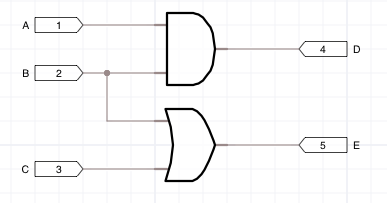
\includegraphics[width=\textwidth]{report_images/img1}
	\caption{\label{fig:figure-name}Circuit diagram for car alarm.}
\end{figure}

As shown in Figure 2, the inputs 'V' and 'D' are tied to the same OR gate, because either the vibration sensor or the door sensor can trigger an alarm if and only if the master switch is activated. Input 'M' is tied to an AND gate to show that the sensors can only trigger an alarm when this input is active. 'S' is the only output and we assume, based on the instructions of this exercise, that this output would be tied to some siren device such as the vehicle's horn or another audio device. The pin assignments for each input and output was given as part of the assignment and is summarized in Table 4.

\begin{table}[h]
\begin{center}
	\begin{tabular}{| l | l | l | l |}
	\hline
	D & V & M & S \\ \hline
	0 & 0 & 0 & 0 \\ \hline
	0 & 0 & 1 & 0 \\ \hline
	0 & 1 & 0 & 0 \\ \hline	
	\end{tabular}
	\caption{\label{tab:table-name}Truth table for the car alarm.}
\end{center}
\end{table}

\begin{table}[h]
\begin{center}
	\begin{tabular}{| l | l | l |}
		\hline
		Bit & Label & Address \\ \hline
		D & Button L & W19 \\ \hline
		V & Switch 15 & R2 \\ \hline
		M & Button R & T17 \\ \hline
		D & LED 7 & V19 \\ \hline
		E & LED 6 & U14 \\ \hline
	\end{tabular}
	\caption{\label{tab:table-name}Input and output bit specification for car alarm.}
\end{center}	
\end{table}

\subsubsection{Results}

The design created in class functioned well and we were able to test each possible combination of inputs and observe their output. We compared these results to our truth table to find that this design worked properly. The results of these trials can be viewed in Figure PICS.

\subsection{Problem 3: Design Our Own Circuit}

\subsubsection{Background and Design Solution}

For our own circuit design, we implemented a simple adder for two 2-bit numbers. Our circuit consists of two full adders with ripple carry. There is assumed to be no carry-in for this system so the carry-in for our least significant bit adder is tied to 0. This design utilizes a component that reuses VHDL code for each full bit adder. This improved our practical understanding of components and streamlined the code process. The two bit numbers x and y are denoted as 'X1', 'X0', 'Y1', and 'Y0' where 1 is the most significant bit and 0 is the least significant bit of the respective number. The output, z, is represented as the bits 'Z1' and 'Z0', where 1 is the most significant bit and 0 is the least significant bit. The carry-out bit is represented by 'cout'. The full adder circuit is displayed in Figure 3 and the 2-bit adder is shown in Figure 4.

\begin{figure}
	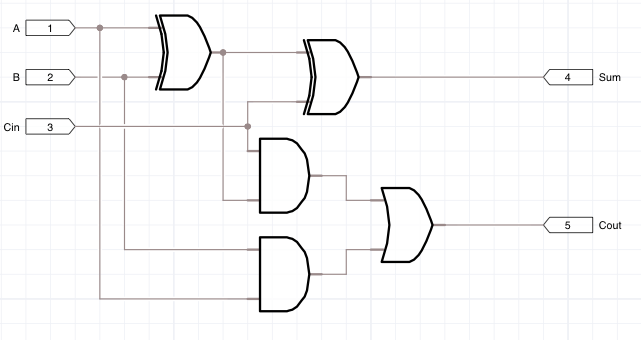
\includegraphics[width=\textwidth]{report_images/img3}
	\caption{\label{fig:figure-name}Circuit diagram for a full adder}
\end{figure}

\begin{figure}
	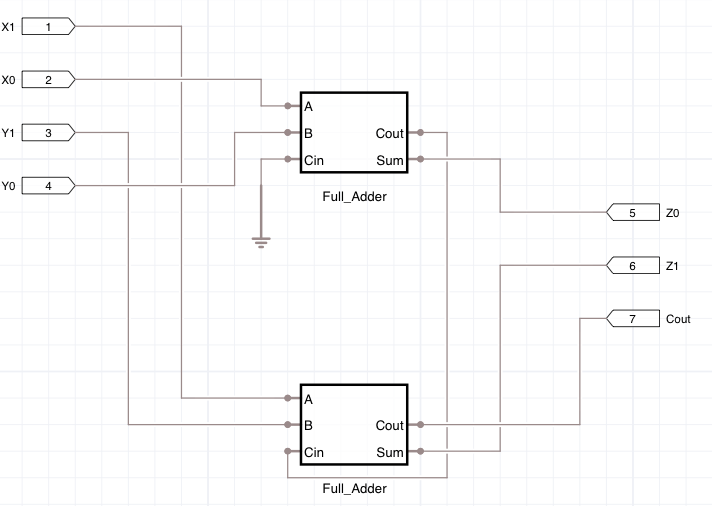
\includegraphics[width=\textwidth]{report_images/img4}
	\caption{\label{fig:figure-name}Circuit diagram for the 2-bit adder implemented for this assignment}
\end{figure}

When completing the pin-mapping for this problem, we prioritize ease-of-use and readability for the user. All bits are entered and displayed with the most significant bit on the right, and each 2-bit number is in a distinct location on the Basys3 board. These assignments are summarized in Table 5. The truth table for the addition of two 2-bit numbers is outlined in Table 6.

\begin{table}[h]
\begin{center}
	\begin{tabular}{| l | l | l |}
		\hline
		Bit & Label & Address \\ \hline
		X0 & Switch 0 & V17 \\ \hline
		X1 & Switch 1 & V16 \\ \hline
		Y0 & Switch 14 & T1 \\ \hline
		Y1 & Switch 15 & R2 \\ \hline
		Z0 & LED 0 & U16 \\ \hline
		Z1 & LED 1 & E19 \\ \hline
		Cout & LED 15 & L1 \\ \hline
	\end{tabular}
	\caption{\label{tab:table-name}Input and output bit specification for adding two 2-bit numbers.}
\end{center}	
\end{table}

\begin{table}[h]
\begin{center}
	\begin{tabular}{| l | l | l | l | l | l | l |}
		\hline
		X1 & X0 & Y1 & Y0 & Cout & Z1 & Z0 \\ \hline
		0 & 0 & 0 & 0 & 0 & 0 & 0 \\ \hline
		0 & 0 & 0 & 1 & 0 & 0 & 1 \\ \hline
		0 & 0 & 1 & 0 & 0 & 1 & 0 \\ \hline
		0 & 0 & 1 & 1 & 0 & 1 & 1 \\ \hline
		0 & 1 & 0 & 0 & 0 & 0 & 1 \\ \hline
		0 & 1 & 0 & 1 & 0 & 1 & 0 \\ \hline
		0 & 1 & 1 & 0 & 0 & 1 & 1 \\ \hline
		0 & 1 & 1 & 1 & 1 & 0 & 0 \\ \hline
		1 & 0 & 0 & 0 & 0 & 1 & 0 \\ \hline
		1 & 0 & 0 & 1 & 0 & 1 & 1 \\ \hline
		1 & 0 & 1 & 0 & 1 & 0 & 0 \\ \hline
		1 & 0 & 1 & 1 & 1 & 0 & 1 \\ \hline
		1 & 1 & 0 & 0 & 0 & 1 & 0 \\ \hline
		1 & 1 & 0 & 1 & 1 & 0 & 0 \\ \hline
		1 & 1 & 1 & 0 & 1 & 0 & 1 \\ \hline
		1 & 1 & 1 & 1 & 1 & 1 & 0 \\ \hline
	\end{tabular}
	\caption{\label{tab:table-name}Truth table for adding two 2-bit numbers}
\end{center}	
\end{table}



\subsubsection{Results}

While this circuit did require our own design, we were able to successfully implement the full adder component in VHDL. This can be viewed in Appendix E. Once again, we were able to view the combination of inputs and resulting output. By comparing these to our truth table, we verified that our design worked properly. These trials are documented in Figure PICS.

\section{Conclusion}

In conclusion, all three design challenges were successfully implemented on the Basys3 board. Moreover, by successfully implementing these designs we have been able to accomplish the primary goal of the lab, which was gaining proficiency with both the Vivado Design Suite and the Digilent Basys3 Development board. The most challenging part of this lab was continuing to fine-tune designs after lab hours. Technically, configuring Vivado to run on a personal computer was quite challenging, but it offered a deeper insight to the overall operations of the design suite, which aided the lab in accomplishing it's mission. Implementing a full program including a component in VHDL also offered a challenge as there are several additional lines of code, such as a USE statement, that needed to be repeated for different entities. At first, this caused a code compilation error, but was corrected. Overall, the results of this lab are as expected, we were able to complete all three tasks, and have gained confidence in using the Vivado Design Suite with the Digilent Basys3.

\pagebreak

\begin{appendices}

\section{Part 1 VHDL Code}

\begin{lstlisting}[language=VHDL]
library IEEE;
use IEEE.STD_LOGIC_1164.ALL;

-- This entity will perform 2 operations with 3 inputs. The result of 
-- each operation will be output to a bit.
entity lab1part1 is
    Port ( a : in STD_LOGIC;
        b : in STD_LOGIC;
        c : in STD_LOGIC;
        d : out STD_LOGIC;
        e : out STD_LOGIC);
	end lab1part1;

architecture Behavioral of lab1part1 is

begin
   	-- Output 'D' will be the result of 'A' AND 'B'
   	d <= a and b;
   	-- Output 'E' will be the result of 'B' OR 'C'
   	e <= b or c;

end Behavioral;
\end{lstlisting}

\section{Part 1 Constraints File}

\begin{figure}[h]
	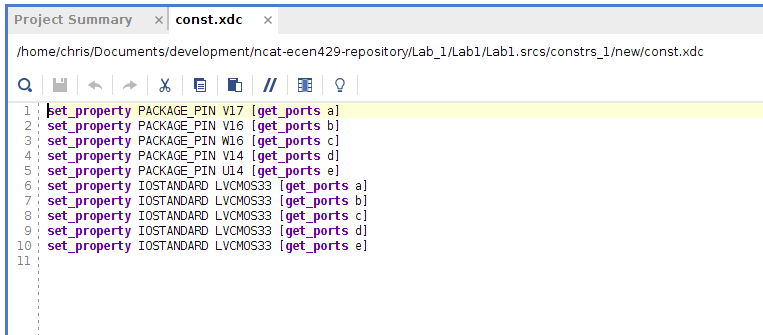
\includegraphics[width=\textwidth]{report_images/img5}
\end{figure}

\section{Part 2 VHDL Code}

\begin{lstlisting}[language=VHDL]
library IEEE;
use IEEE.STD_LOGIC_1164.ALL;

-- This entity has 3 inputs, the master switch, vibration sensor, and door sensor
-- described in the car alarm problem. The siren is the only output.
entity lab1part2 is
    Port ( m : in STD_LOGIC;
           v : in STD_LOGIC;
           d : in STD_LOGIC;
           s : out STD_LOGIC);
end lab1part2;

architecture Behavioral of lab1part2 is

-- tmp1 is required to carry the sensor state from the sensor OR gate to the master
-- switch AND gate
signal tmp1 : STD_LOGIC;

begin

    --tmp1 tells whether or not a sensor is active
    tmp1 <= v or d;
    --'S' will be set to high when both the master switch AND a sensor are active
    s <= m and tmp1;

end Behavioral;
\end{lstlisting}

\pagebreak

\section{Part 2 Constraints File}

\begin{figure}[h]
	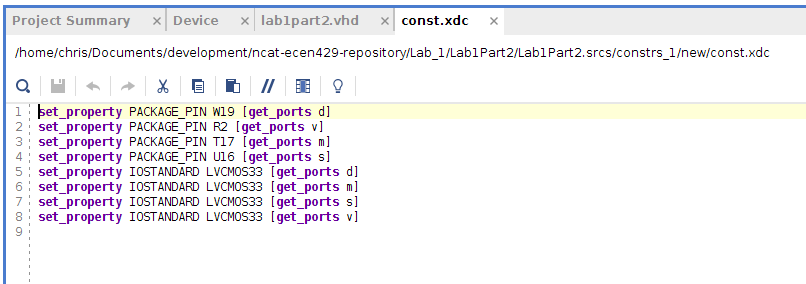
\includegraphics[width=\textwidth]{report_images/img6}
\end{figure}

\section{Part 3 VHDL Code}

\begin{lstlisting}[language=VHDL]
library IEEE;
use IEEE.STD_LOGIC_1164.ALL;

-- The following two lines declare the full_adder, which will later be
-- used as acomponent. The full adder takes two 1-bit numbers and a 
-- carry-in, and adds them.
entity full_adder is port(a, b, cin: in STD_LOGIC; sum, cout :out STD_LOGIC);
end entity full_adder;

architecture adder_arch of full_adder is
begin
    -- The comparison of a, b, and cin will determine the output
    process(a, b, cin);
    begin
    -- Every possible case is documented and outputs are assigned.
    if (a = '0' and b = '0' and cin = '0') then (cout <= '0' & sum <= '0');
		elsif (a = '0' and b = '0' and cin = '1') 
			then (cout <= '0' & sum <= '1');
		elsif (a = '0' and b = '1' and cin = '0') 
			then (cout <= '0' & sum <= '1');
		elsif (a = '0' and b = '1' and cin = '1') 
			then (cout <= '1' & sum <= '0');
		elsif (a = '1' and b = '0' and cin = '0') 
			then (cout <= '0' & sum <= '1');
		elsif (a = '1' and b = '0' and cin = '1') 
			then (cout <= '1' & sum <= '1');
		elsif (a = '1' and b = '1' and cin = '0') 
			then (cout <= '1' & sum <= '0');
		elsif (a = '1' and b = '1' and cin = '1') 
			then (cout <= '1' & sum <= '1');
	end if;
	end process;
end architecture adder_arch;

library IEEE;
use IEEE.STD_LOGIC_1164.ALL;

-- This entity is the top-level entity of this program. It will add two 
-- 2-bit numbers. The carry-in for the least significant bit addition 
-- is assumed to be 0 for this closed system.
entity lab1part3 is
    Port ( x1 : in STD_LOGIC;
           x0 : in STD_LOGIC;
           y1 : in STD_LOGIC;
           y0 : in STD_LOGIC;
           z1 : out STD_LOGIC;
           z0 : out STD_LOGIC;
           cout : out STD_LOGIC);
end lab1part3;

architecture adder of lab1part3 is
-- This signal is needed to relay the carry-out of the least significant
--  bit operation to the carry-in of the most significant bit operation.
signal tmpcarry:STD_LOGIC;

-- This declares a full_adder component based on the entity above. This 
-- declaration is only needed once in order to use the full_adder twice.
component full_adder port(a,b,cin : in STD_LOGIC; sum, cout : out STD_LOGIC);
end component full_adder;

begin
    -- This adder performs the least significant bit operation
    component_0 : full_adder port map (x0, y0, '0', z0, tmpcarry);
    -- This adder performs the most significant bit operation
    component_2 : full_adder port map (x1, y1, tmpcarry, z1, cout);

end adder;
\end{lstlisting}

\section{Part 3 Constraints File}

\begin{figure}[h]
	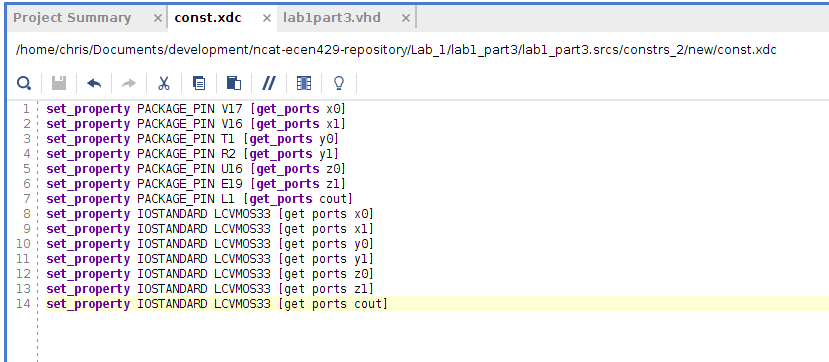
\includegraphics[width=\textwidth]{report_images/img7}
\end{figure}

\end{appendices}

\end{document}
